\documentclass[11pt]{article}
\usepackage[margin=1in]{geometry}
\usepackage{graphics, graphicx, cite, fancybox, setspace}
\usepackage{amsfonts, amssymb, amsmath, latexsym, epic, eepic, url,enumitem}
\usepackage{wrapfig, subfigure}
\usepackage{multirow}
\usepackage{palatino}
\usepackage[mathscr]{euscript}
\usepackage{amsfonts}
\usepackage[bf]{caption}
\usepackage{dcolumn}
\usepackage[numbers]{natbib}
\usepackage[usenames,dvipsnames]{color}
%\usepackage[normalem]{ulem}
%\usepackage{enumitem}
\usepackage{acronym}
%\usepackage[centertags]{amsmath}
%\usepackage{amsfonts,amssymb}
\usepackage{accents}
\usepackage{tikz}
\usetikzlibrary{shapes,arrows}
% Default fixed font does not support bold face
\DeclareFixedFont{\ttb}{T1}{txtt}{bx}{n}{12} % for bold
\DeclareFixedFont{\ttm}{T1}{txtt}{m}{n}{12}  % for normal

% Custom colors
\usepackage{color}
\definecolor{deepblue}{rgb}{0,0,0.5}
\definecolor{deepred}{rgb}{0.6,0,0}
\definecolor{deepgreen}{rgb}{0,0.5,0}

\usepackage{listings}

% Python style for highlighting
\newcommand\pythonstyle{\lstset{
language=Python,
basicstyle=\ttm,
otherkeywords={self},             % Add keywords here
keywordstyle=\ttb\color{deepblue},
emph={MyClass,__init__},          % Custom highlighting
emphstyle=\ttb\color{deepred},    % Custom highlighting style
stringstyle=\color{deepgreen},
frame=tb,                         % Any extra options here
showstringspaces=false            % 
}}


% Python environment
\lstnewenvironment{python}[1][]
{
\pythonstyle
\lstset{#1}
}
{}

% Python for external files
\newcommand\pythonexternal[2][]{{
\pythonstyle
\lstinputlisting[#1]{#2}}}

% Python for inline
\newcommand\pythoninline[1]{{\pythonstyle\lstinline!#1!}}
%\renewcommand{\baselinestretch}{1.1}
%
\newcommand{\molar}[1]{\underaccent{\bar}{#1}}
\def\Vm{\molar{V}}
%\renewcommand{\figurename}{Algorithm}
\newcommand{\cfa}[1]{\color{red}{#1}\color{black}}
\newcommand{\eve}[1]{\color{blue}{#1}\color{black}}
\newcommand{\uu}[1]{{\boldsymbol #1}}
\newcommand{\tpd}[3]
{\left(\frac{\partial {#1}}{\partial {#2}}\right)_{#3}}
\def\ttau{\uu{\tau}}
\def\bb{\uu{b}}
\def\nb{\uu{n}}
\def\pb{\uu{p}}
\def\wb{\uu{w}}
\def\xb{\uu{x}}
\def\yb{\uu{y}}
\def\vb{\uu{v}}
\def\zb{\uu{z}}
\def\Xb{\uu{X}}
\def\etab{\uu{\eta}}
\def\thetab{\uu{\theta}}
\def\lambdab{\uu{\lambda}}
\def\gammab{\uu{\gamma}}
\def\taub{\uu{\tau}}
\def\phib{\uu{\phi}}
\def\psib{\uu{\psi}}
\def\nub{\uu{\nu}}
\def\nablab{\uu{\nabla}}
\def\varphib{\uu{\varphi}}
\def\Ab{\uu{A}}
\def\Bb{\uu{B}}
\def\Gb{\uu{G}}
\def\Vb{\uu{V}}
\def\Fb{\uu{F}}
\def\Jb{\uu{J}}
\def\Rb{\uu{R}}
\def\Tb{\uu{T}}
\def\Mb{\uu{M}}
\def\rb{\uu{r}}
\tikzstyle{decision} = [diamond, draw, fill=blue!20, 
    text width=4.5em, text badly centered, node distance=3cm, inner sep=0pt]
\tikzstyle{block} = [rectangle, draw, fill=blue!20, 
    text width=7em, text centered, rounded corners, minimum height=4em]
\tikzstyle{gblock} = [rectangle, draw, fill=green!20,
    text width=7em, text centered, rounded corners, minimum height=4em]
\tikzstyle{line} = [draw, -latex']
\tikzstyle{cloud} = [draw, ellipse,fill=red!20, node distance=3cm,
    minimum height=2em]
\hyphenation{mol-e-cules}
\newenvironment{packed_item}{
\begin{itemize}
  \setlength{\itemsep}{0pt}
  \setlength{\parskip}{0pt}
  \setlength{\parsep}{0pt}
}{\end{itemize}}

\newenvironment{packed_enum}{
\begin{enumerate}
  \setlength{\itemsep}{0pt}
  \setlength{\parskip}{0pt}
  \setlength{\parsep}{0pt}
}{\end{enumerate}}

\renewcommand\thesection{\Alph{section}}

\newif \ifshowsolutions
\showsolutionstrue
\showsolutionsfalse

\begin{document}

\begin{centering}
{\sc D\ R\ E\ X\ E\ L\ \ \ U\ N\ I\ V\ E\ R\ S\ I\ T\ Y}\\
College of Engineering\\
ENGR 131 -- Programming \\
Winter 18-19\\
A Suggested Programming Exercise:  Computing Pure-Species Vapor Pressures\\
Cameron F. Abrams -- cfa22@drexel.edu\\
Department of Chemical and Biological Engineering\\
\ifshowsolutions
\textcolor{blue}{S\ O\ L\ U\ T\ I\ O\ N\ S}\\
\fi
\end{centering}

\section*{Summary}
In this assignment, you'll develop a Python program to compute the {\bf vapor pressure} $P^{\rm vap}$ at a specified temperature $T$ for any pure substance, using the general Peng-Robinson equation of state.  The computational learning outcome of this assignment is the development of a {\em convergent algorithm} for implicit solution.  The Python skills that are used here include {\bf looping}, {\bf conditionals}, {\bf arrays}, and {\bf functions}.

\section*{Background and Relevant Equations}
At a given temperature $T$, the vapor pressure $P^{\rm vap}$ of a pure species is the pressure at which the pure liquid and pure vapor are in equilibrium with each other.  (When $P^{\rm vap}$ is taken as 1 atmosphere, $T$ is the ``normal boiling point'' temperature.)  This kind of information is important in many situations where fluids are being processed.  At a given temperature $T$, we know a fluid will be in the vapor phase for pressures below $P^{\rm vap}(T)$ or in the liquid phase at pressures above $P^{\rm vap}(T)$.  But $P^{\rm vap}(T)$ is not a universal property: at a given temperature, different substances can have very different $P^{\rm vap}$, and some might not have any $P^{\rm vap}$ at all!  (If $T$ is greater than a substance's ``critical temperature'' $T_c$, there is no pressure at which liquid can be made to form.)  So this situation motivates engineers to find ways to predict $P^{\rm vap}$ mathematically, or at least use as much information as possible from careful experiments that have already been done.  How can we do this?

First, recognize that we need to use physical laws that allow us to {\em interrelate} variables like $T$ and $P$.  For instance, you are already familiar with the ideal gas law, which you may have seen written in a variety of algebraically identical ways, e.g.,
%
\begin{equation}\label{eq:ideal-gas-law}
PV = n R T\ \ \ \ \mbox{or}\ \ \ \ \ P = \frac{RT}{\Vm}\ \ \ \ \ \mbox{or}\ \ \ \ \rho = \frac{P}{R T},
\end{equation}
%
where $V$ is volume, $n$ is number of moles, $R$ is the gas constant (8.314$\times$10$^{-5}$~bar-m$^3$/mol-K), $\rho$ is molar density $n/V$, and $\Vm$ is molar volume $V/n$.  This equation of state says, among other things, that at a given temperature $T$ and pressure $P$, a substance can have one and only one density $\rho$.  Clearly, then, the ideal gas law is useless in helping us predict whether or not a substance has a vapor pressure at a given $T$.  After all, in such a situation, our substance simultaneously has {\em two different densities} (a low-density vapor and high-density liquid) at one given $T$ and $P=P^{\rm vap}$.   

This deficiency of the ideal gas law led thermodynamicists (many of whom were industrial chemical and mechanical engineers) to develop more sophisticated ``real-gas'' equations of state.  One goal of these equations of state is, along with a thermodynamic recipe we will learn about here, to allow one to predict whether or not a {\em particular} pure substance can have a vapor pressure at any given temperature. Here, we will work with the industry-standard Peng-Robinson (``PR'') equation of state:
%
\begin{align}
%\label{eq:pr-main} P & = \frac{RT}{\Vm-b} - \frac{a(T)}{\Vm(\Vm+b)+b(\Vm-b)},\\
\label{eq:pr-Z} Z^3+c_2 Z^2 + c_1 Z + c_0 & = 0,\\
\label{eq:prZ-Zdef}\mbox{where}\ \ \ Z & \equiv \frac{P\Vm}{RT},\\
\label{eq:c2} c_2 & = -1 + B,\\
\label{eq:c1} c_1 & = A - 3B^2 - 2B,\\
\label{eq:c0} c_0 & = -AB + B^2 + B^3,\\
%\label{eq:prZ-A} A & = a P/(RT)^2,\\
%\label{eq:prZ-B} B & = bP/RT,\\
\label{eq:pr-kappa} \kappa & = 0.37464 + 1.5422\omega -0.26992\omega^2,\\
\label{eq:prZ-A} A & = 0.45724\left(\frac{P}{P_c}\right)\left(\frac{T_c}{T}\right)^2\left[1+\kappa\left(1-\sqrt{\frac{T}{T_c}}\right)\right]^2,\ \ \mbox{and}\\
\label{eq:prZ-B} B & = 0.07780\left(\frac{T_c}{T}\right)\left(\frac{P}{P_c}\right).
\end{align}
%
$T_c$ is the critical temperature, $P_c$ is the critical pressure, and $\omega$ is the acentricity factor; all of these are substance-specific constants.  (See Table~\ref{tbl:data} for a very small sample of this data for three selected substances.)  $Z$ is called the ``compressibility factor''.

Why is this equation of state so complicated?  Eq.~\ref{eq:pr-Z} is {\em cubic} in $Z$; its solutions are values of $Z$ for which this third-order polynomial vanishes.  These are referred to as ``roots'' of the cubic.  PR always has at least one real root, and for {\em some} values of its coefficients ($c_2$, $c_1$, and $c_0$), it can have {\em three} real roots.  In such a case, the lowest root $Z_L$ is associated with the {\em liquid} phase (since it has a {\em low} compressibility) and the highest root $Z_V$ is associated with the {\em vapor} phase (since it has a {\em high} compressibility).  The middle root is always ignored.  So, this equation is complicated so that it has the ability to predict {\em coexistence} of liquid and vapor phases of the same substance.

How do you use such an equation? If given the identity of a substance (its $T_c$, $P_c$, and $\omega$), a temperature $T$, and a pressure $P$, PR can tell us if there is a single phase (only one root $Z$) or two phases ($Z_L$ and $Z_V$).  If we find two roots, how do we know $P$ is $P^{\rm vap}$?  The answer comes from thermodynamics, which requires that, at the given $T$ and $P$, the vapor and liquid phases also have the {\em same molar Gibbs free energy}.  Don't worry about the deep meaning here; we'll just focus on the result.  The result is that, at $T$, we have to find that one unique value of $P$ for which a {\em second} condition is met.  That second condition is the {\em equality of fugacities}.  The fugacity $f$ of a substance that obeys PR is given by
%
\begin{equation}\label{eq:fugacity}
\ln\frac{f}{P} = Z - 1 - \ln(Z-B) - \frac{A}{2\sqrt{2}B}\ln\left[\frac{Z+(1+\sqrt{2})B}{Z+(1-\sqrt{2})B}\right]
\end{equation}
%
$A$ and $B$ are defined in Eq.~\ref{eq:prZ-A} and~\ref{eq:prZ-B}, respectively.  

\underline{Here's the bottom line:}  Eq.~\ref{eq:pr-Z} through~\ref{eq:fugacity} provide a framework for determining whether or not a particular substance (represented by $T_c$, $P_c$, and $\omega$) has a $P^{\rm vap}$ at any given $T$.  Let's now think about how you can find this particular value of $P$.  It looks like you just have to guess a value for $P$ and run it (along with $T$, $T_c$, $P_c$, and $\omega$) through all these equations to see if you get two roots $Z_L$ and $Z_V$ which, when individually used in Eq.~\ref{eq:fugacity}, give the same value for $f$.  If your guess does {\em not}, then you should have a way to ``adjust'' your guess and try again.  Pretty quickly, we see that a computer program is the right way to do this.

So, to write a program to compute $P^{\rm vap}(T)$, we need to have an algorithm that will {\em converge} on the right value of $P$. We turn to this algorithm next.

\section*{The Vapor Pressure Calculation Algorithm}

The algorithm for computing $P^{\rm vap}$ that you will implement in this assignment is shown in Fig.~\ref{fig:algo1}.  This is a {\em convergent} algorithm, designed to correct a current guess for $P$ to drive toward the stopping condition. The stopping condition encodes the idea that we want the two fugacities, $f_V$ and $f_L$, to be equal; in reality, we will settle for them being ``close enough'', defined precisely as $|1-\frac{f_L}{f_V}|<\epsilon$, where we choose how small we would like $\epsilon$ to be (10$^{-6}$ is not a bad choice).
%
\begin{figure}
\begin{center}
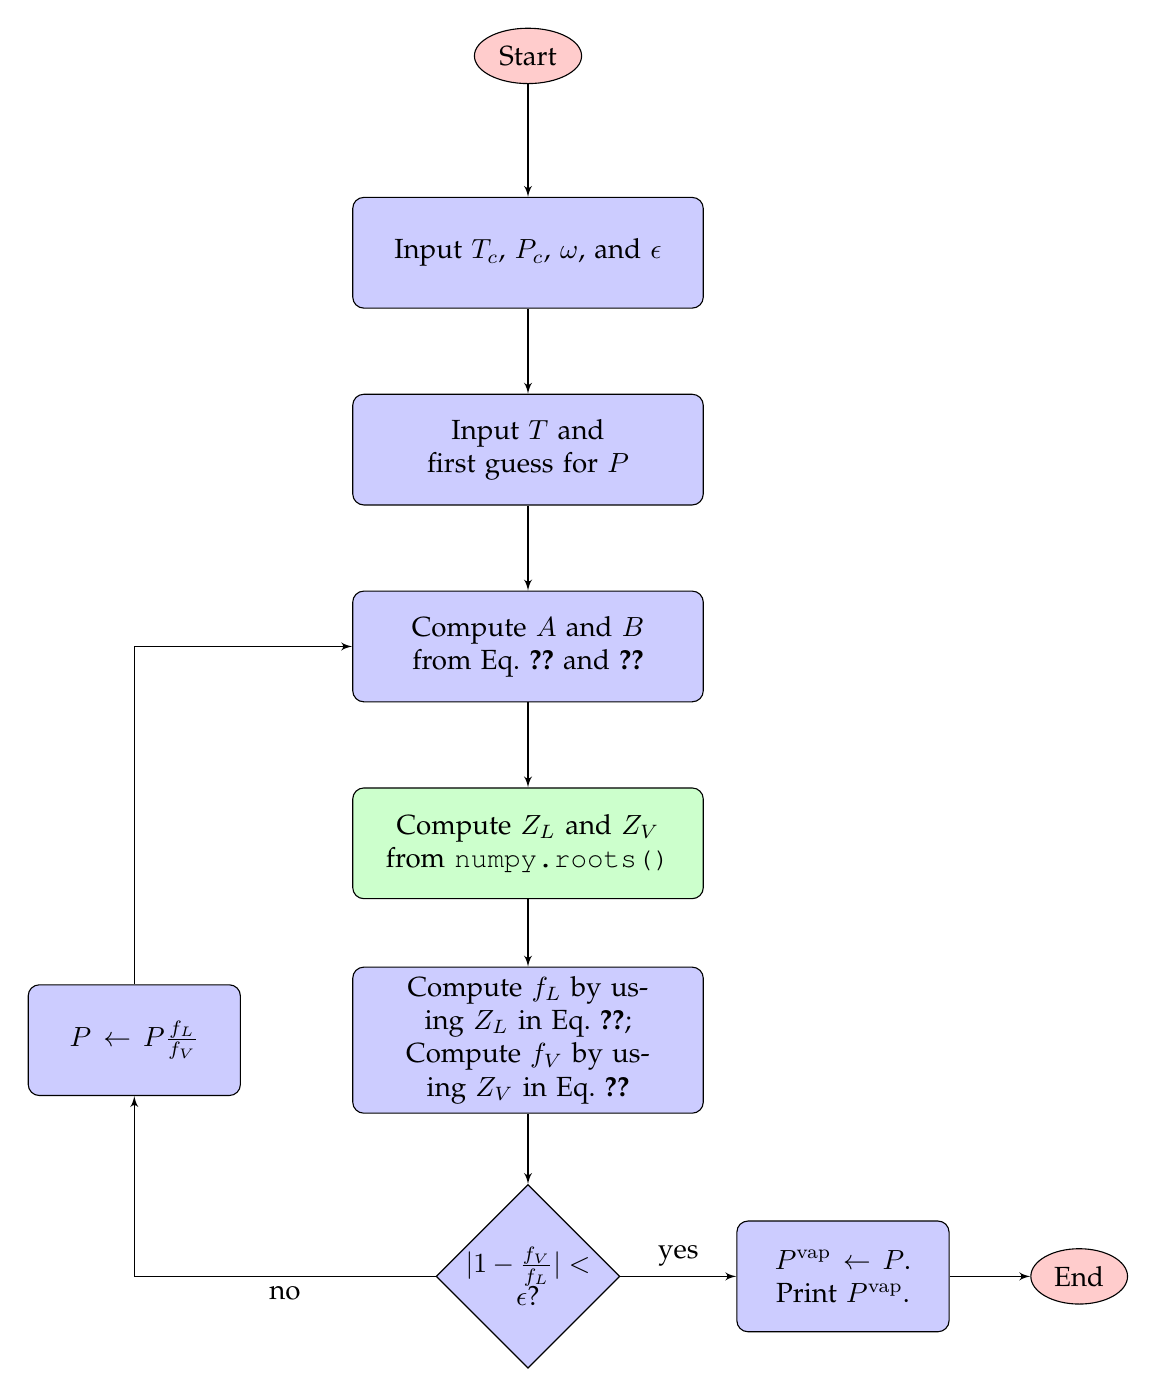
\begin{tikzpicture}[node distance = 2.5cm, auto]
\node [cloud] (start) {Start};
\node [block, below of=start, text width=12em] (init) {Input $T_c$, $P_c$, $\omega$, and $\epsilon$};
\node [block, below of=init, text width=12em] (setup) {Input $T$ and first guess for $P$};
%\node [block, below of=setup, text width=12em] (identify) {Compute $a$ and $b$ from Eq.~\ref{eq:pr-a} and \ref{eq:pr-b}};
\node [block, below of=setup, text width=12em] (AB) {Compute $A$ and $B$ from Eq.~\ref{eq:prZ-A} and~\ref{eq:prZ-B}};
\node [gblock, below of=AB, text width=12em] (Z) {Compute $Z_L$ and $Z_V$ from {\tt numpy.roots()}};
%\node [gblock, right of=Z, node distance=4cm] (algo) {Algorithms 2 \& 3};
\node [block, below of=Z, text width=12em] (FL) {Compute $f_L$ by using $Z_L$ in Eq.~\ref{eq:fugacity};\\
Compute $f_V$ by using $Z_V$ in Eq.~\ref{eq:fugacity}};
\node [decision, below of=FL] (q) {$|1-\frac{f_V}{f_L}|<\epsilon$?};
\node [block, left of=FL, node distance=5cm] (adjust) {$P\gets P\frac{f_L}{f_V}$};
\node [block, right of=q, node distance=4cm] (stop) {$P^{\rm vap} \gets P$.  Print $P^{\rm vap}$.};
\node [cloud, right of=stop, node distance=3cm] (end) {End};
\path [line] (start) -- (init);
\path [line] (init) -- (setup);
%\path [line] (setup) -- (identify);
\path [line] (setup) -- (AB);
\path [line] (AB) -- (Z);
\path [line] (Z) -- (FL);
\path [line] (FL) -- (q);
\path [line] (q) -| node [near start] {no} (adjust);
\path [line] (adjust) |- (AB);
\path [line] (q) -- node {yes} (stop);
\path [line] (stop) -- (end);
%\path [line] (AB) -| (algo);
%\path [line] (algo) -- (Z);
\end{tikzpicture}
\end{center}
\caption{\label{fig:algo1} Algorithm 1.  Vapor-pressure calculation using the PR equation.}
\end{figure}

\subsection*{Roots of a cubic using {\tt numpy.roots()}}
The green block in Fig.~\ref{fig:algo1} indicates that we need a more detailed explanation to compute $Z_V$ and $Z_L$.  Here, we realize we are solving for roots of a cubic polynomial.  To do this, we are going to use a the {\tt numpy.roots()} function.  This function takes a single array argument of coefficients of a polynomial.  For Eq.~\ref{eq:pr-Z} through~\ref{eq:c0}, python code to find the roots would look like this:
\begin{python}
from numpy import roots
# [code to compute A, B]
coeff = [ 1, -1 + B, A - 3*B*B - 2*B, -A*B + B*B + B*B*B ]
Z = roots(coeff)
\end{python}
Here {\tt Z} is an array with three elements; if there are three real roots, they will be in {\em descending numerical order}.  If there is only one real root, it will be element {\tt 0}.  To determine whether or not the third root is complex or a pure real number, we need to look at its imaginary component:
\begin{python}
ZV = Z[0].real
ZL = 0
if ( Z[2].imag != 0 ):
   print "Only one root found"
else:
   ZL = Z[2].real
\end{python}

\begin{table}
\begin{center}
\caption{\label{tbl:data} Critical temperatures, pressures, and acentricity factors for selected pure species (extracted from R. C. Reid, J. M. Prausnitz, and B. E. Poling, 1987, {\it The Properties of Gases and Liquids}, 4$^{\rm th}$ Ed., New York: McGraw-Hill).}
\begin{tabular}{lr@{.}lr@{.}lr@{.}l}
Species & \multicolumn{2}{c}{$P_c$ (bar)} &\multicolumn{2}{c}{$T_c$ (K)} & \multicolumn{2}{c}{$\omega$}\\\hline
$n$-butane &  38&0 & 425&2 & 0&199\\ 
ethanol &  61&4 & 513&9 & 0&644\\
ammonia &  113&5 & 405&5 & 0&25\\
sulfur dioxide & 78&83 & 430&8 & 0&251\\
\end{tabular}
\end{center}
\end{table}

\clearpage

\section*{The Assignment}

\begin{enumerate}
\item Write a Python program that can print out values of $A$ and $B$ (Eq.~\ref{eq:prZ-A} and~\ref{eq:prZ-B}, respectively) if values of $T$, $P$, $T_c$, $P_c$, $\omega$ are provided; use it to compute $A$ and $B$ for $n$-butane at 1 bar and 298.15 K.

\ifshowsolutions
\textcolor{blue}{Solution.}  The program appears below. 

\begin{python}
Tc = 425.2
Pc = 38.0
omega = 0.199
P = 1
T = 298.15
kappa = 0.37464 + 1.54226*omega - 0.26992*omega*omega
A = 0.45724*(P/Pc)*(Tc/T)**2*(1+kappa*(1-(T/Tc)**(0.5)))**2
B = 0.07780*(Tc/T)*(P/Pc)
print "A = {0:.8f}, B = {1:.8f}".format(A,B)
print "Program ends."
\end{python}
This program produces the following output:
\begin{verbatim}
A = 0.03010351, B = 0.00291981
Program ends.
\end{verbatim}
\clearpage
\fi

\item Modify this program to use $A$ and $B$ to compute the coefficients of the cubic polynomial $c_2$, $c_1$, and $c_0$ and place these in four dimensional array of coefficients (where the coefficient on $Z^3$ is 1).  Use them in a call to {\tt numpy.roots()} to return an array of roots.  Use this new program to determine $Z_V$ And $Z_L$ for $n$-butane at 1 bar and 298.15 K, and again at 1 bar and 800 K.  (Do you have two real roots at 800 K?)

\ifshowsolutions
\textcolor{blue}{Solution.}\  The program appears below.  We have used the code given in the problem description.
\begin{python}
from numpy import roots
Tc = 425.2
Pc = 38.0
omega = 0.199
P = 1
T = 298.15
kappa = 0.37464 + 1.54226*omega - 0.26992*omega*omega
A = 0.45724*(P/Pc)*(Tc/T)**2*(1+kappa*(1-(T/Tc)**(0.5)))**2
B = 0.07780*(Tc/T)*(P/Pc)
coeff = [ 1, -1 + B, A - 3*B*B - 2*B, -A*B + B*B + B*B*B ]
Z = roots(coeff)
ZV = Z[0].real
ZL = 0
if ( Z[2].imag != 0 ):
   print "Only one root found"
else:
   ZL = Z[2].real
print "ZV = {0:.8f}, ZL = {1:.8f}".format(ZV,ZL)
print "Program ends."
\end{python}

For {\tt T = 298.15}, this program generates the following output:
\begin{verbatim}
A = 0.03010351, B = 0.00291981
ZV = 0.97223359, ZL = 0.00389535
Program ends.
\end{verbatim}

For {\tt T = 800}:
\begin{verbatim}
Only one root found
A = 0.00191539, B = 0.00108818
ZV = 0.99917745, ZL = 0.00000000
Program ends.
\end{verbatim}
\clearpage
\fi

\item Insert a function into your program that computes the {\em dimensionless} fugacity $f/P$ (defined in Eq.~\ref{eq:fugacity}).  Use this program to compute $f/P$ at each of $Z_L$ and $Z_V$ for $n$-butane at 298.15 K with a guess of $P$ = 1 bar.

\ifshowsolutions
\textcolor{blue}{Solution.}\ The {\tt def} statement below defines this new function.  Note that we have to import the reserved math functions {\tt exp}, {\tt log}, and {\tt sqrt}.
\begin{python}
from math import exp, log, sqrt
from numpy import roots
def pr_fug (z, A, B):
   r2 = sqrt(2)
   arg = z-1-log(z-B)-A/(2*r2*B)*log((z+(1+r2)*B)/(z+(1-r2)*B))
   return exp(arg)
Tc = 425.2
Pc = 38.0
omega = 0.199
P = 1
T = 298.15
kappa = 0.37464 + 1.54226*omega - 0.26992*omega*omega
A = 0.45724*(P/Pc)*(Tc/T)**2*(1+kappa*(1-(T/Tc)**(0.5)))**2
B = 0.07780*(Tc/T)*(P/Pc)
coeff = [ 1, -1 + B, A - 3*B*B - 2*B, -A*B + B*B + B*B*B ]
Z = roots(coeff)
ZV = Z[0].real
ZL = 0
if ( Z[2].imag != 0 ):
   print "Only one root found"
else:
   ZL = Z[2].real
print "A = {0:.8f}, B = {1:.8f}".format(A,B)
print "ZV = {0:.8f}, ZL = {1:.8f}".format(ZV,ZL)
print "f/P(ZV) = {0:.8f}".format(pr_fug(ZV,A,B))
if ( ZL > 0 ):
    print "f/P(ZL) = {0:.8f}".format(pr_fug(ZL,A,B))
print "Program ends."
\end{python}

This program generates the following outputs:
\begin{verbatim}
A = 0.03010351, B = 0.00291981
ZV = 0.97223359, ZL = 0.00389535
f/P(ZV) = 0.97290365
f/P(ZL) = 2.26069776
Program ends.
\end{verbatim}

\clearpage
\fi

\item {\bf Implement Algorithm 1.}  
\begin{enumerate}
\item Add variables {\tt crit} and {\tt niter} to the main program.  {\tt crit} is where you will store $f_L/f_V$.  Initialize it to 0.  {\tt niter} will keep track of how many iterations the algorithm has run.  
\item Add the variable {\tt maxiter} and initialize it to 1000.  
\item Embed the lines beginning with {\tt A =}... through the calculation/check of the roots in a {\tt while} loop that executes so long as $\left|1-f_L/f_V\right|>\epsilon$ {\bf and} {\tt niter < maxiter}.  
\item In the body of this loop, near the end, add a line to compute {\tt crit} (that calls the fugacity function twice), another that updates the pressure using {\tt crit}, and another to update {\tt niter}.
\item In the body of the loop, add an {\tt exit()} call to the conditional branch if only one root is found.
\item In the body of the loop, immediately prior to the {\tt niter} update, output the current pressure and the number of iterations.
\item Outside and after the {\tt while} loop, output the current value of pressure; this should be $P^{\rm vap}$.
\item Use this program to compute $P^{\rm vap}$ of $n$-butane at 278.15 K, using 1 bar as an initial guess.
\end{enumerate}

\ifshowsolutions
\textcolor{blue}{Solution.}\ In the code below, each line that addresses an item above is labeled with a comment indicating which item it addresses.
\begin{python}
from math import exp, log, sqrt
from numpy import roots
def pr_fug (z, A, B):
   r2 = sqrt(2)
   arg = z-1-log(z-B)-A/(2*r2*B)*log((z+(1+r2)*B)/(z+(1-r2)*B))
   return exp(arg)
Tc = 425.2
Pc = 38.0
omega = 0.199
ep = 1.e-6
maxiter = 1000 # (b)
P = 1
T = 298.15
kappa = 0.37464 + 1.54226*omega - 0.26992*omega*omega
crit = 0 # (a)
niter = 0 # (a)
while ( abs(1-crit) > ep and niter < maxiter ):  # (c)
   A = 0.45724*(P/Pc)*(Tc/T)**2*(1+kappa*(1-(T/Tc)**(0.5)))**2
   B = 0.07780*(Tc/T)*(P/Pc)
   coeff = [ 1, -1 + B, A - 3*B*B - 2*B, -A*B + B*B + B*B*B ]
   Z = roots(coeff)
   ZV = Z[0].real
   ZL = 0
   if ( Z[2].imag != 0 ):
      print "Only one root found"
      exit() # (e)
   else:
      ZL = Z[2].real
   crit = pr_fug(ZL,A,B)/pr_fug(ZV,A,B) # (d)
   P = P * crit # (d)
   print "iter = {0:d}, Pressure = {1:.8f} bar".format(niter,P)
   niter = niter + 1  # (d)
print "Pvap = {0:0.8f} bar".format(P)
print "Program ends."
\end{python}

This program outputs the following.
\begin{verbatim}
iter = 0, Pressure = 2.32366049 bar
iter = 1, Pressure = 2.42447399 bar
iter = 2, Pressure = 2.43244712 bar
iter = 3, Pressure = 2.43307957 bar
iter = 4, Pressure = 2.43312975 bar
iter = 5, Pressure = 2.43313373 bar
iter = 6, Pressure = 2.43313405 bar
Pvap = 2.43313405 bar
Program ends.
\end{verbatim}

\clearpage
\fi

\item Modify your program to allow it to loop over temperatures between specified limits to perform a series of vapor-pressure calculations at regular intervals along $T$ for $T<T_c$.  Have your program display a plot of $\ln(P^{\rm vap})$ (between -20 and 5) vs. $1/T$ (between 0.002 and 0.010) using {\tt matplotlib}.  Use this program to generate such a plot for ammonia, for $150 \le T \le 390$~K. 

\ifshowsolutions
\textcolor{blue}{Solution.}\ The version of the program that makes this plot appears below.  We have introduced the {\tt T\_list[]} and {\tt P\_list[]} arrays.  We also introduced a control scheme that continues the calculation along $T$ so long as $Z_L$ is not zero upon the beginning of any iteration. $Z_L$ = 0 is the condition signifying that there are not two real roots, but only one. The plot commands appear at the end.

\begin{python}
from math import exp, log, sqrt
from numpy import roots
import matplotlib.pyplot as plt
def pr_fug (z, A, B):
   r2 = sqrt(2)
   arg = z-1-log(z-B)-A/(2*r2*B)*log((z+(1+r2)*B)/(z+(1-r2)*B))
   return exp(arg)
lab='ammonia'
Tc = 405.5                                                                                                                                                                               
Pc =113.5                                                                                                                                                                                
omega = 0.250                                                                                                                                                                            
ep = 1.e-6                                                                                                                                                                               
maxiter = 1000                                                                                                                                                                           
P = 1                                                                                                                                                                                    
T = 150
dT = 10
kappa = 0.37464 + 1.54226*omega - 0.26992*omega*omega
T_list=[]
P_list=[]
ZL=ep
while ( ZL > 0 and T < Tc ):
   crit = 0
   niter = 0
   while ( ZL > 0 and abs(1-crit) > ep and niter < maxiter ):
      A = 0.45724*(P/Pc)*(Tc/T)**2*(1+kappa*(1-(T/Tc)**(0.5)))**2
      B = 0.07780*(Tc/T)*(P/Pc)
      coeff = [ 1, -1 + B, A - 3*B*B - 2*B, -A*B + B*B + B*B*B ]
      Z = roots(coeff)
      ZV = Z[0].real
      if ( Z[2].imag != 0 ):
         ZL = 0
      else:
         ZL = Z[2].real
      if ( ZL > 0 ):
         crit = pr_fug(ZL,A,B)/pr_fug(ZV,A,B)
         P = P * crit
         niter = niter + 1
   if ( ZL > 0 ):
      print "T = {0:.3f} K, P = {1:.8f} bar".format(T,P) 
      T_list.append(1.0/T)
      P_list.append(log(P))
      T = T + dT
plt.plot(T_list,P_list,label=lab)
plt.legend()
plt.ylabel('ln Pvap(bar)')
plt.xlabel('1/T(K)')
plt.ylim([-20,5])
plt.xlim([0.002,0.010])
plt.savefig("my-ammonia.png")
\end{python}

The plot is shown in Fig.~\ref{fig:pvap}.

\begin{figure}[ht]
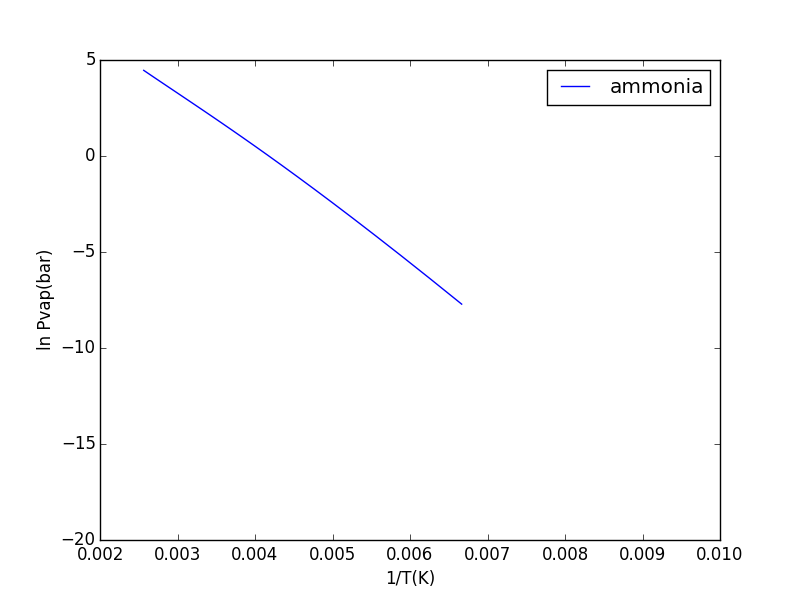
\includegraphics[width=0.75\textwidth]{my-ammonia.png}
\caption{\label{fig:pvap} Vapor pressures vs temperatures for ammonia, computed using the Peng-Robinson equation of state.}
\end{figure}

\fi

\item Write a Python program that will generate a {\em single} plot with vapor pressure curves for n-butane, ethanol, ammonia, and sulfur dioxide, where each substance is listed in an input file, one substance per line, with the following format:
%
\begin{verbatim}
name Tc(K) Pc(bar) omega Tmin(K)
\end{verbatim}
%
The temperature ranges for each curve are as follows:
\begin{enumerate}
\item $n$-butane for $100 \le T \le 400$~K.
\item ethanol for $200 \le T \le 490$~K.
\item ammonia for $150 \le T \le 390$~K.
\item sulfur dioxide for $253.15 \le T \le 413.15$~K.
\end{enumerate}

\ifshowsolutions
\textcolor{blue}{Solution.}\ First, the input file looks like this (I called it '{\tt properties.dat}'):
%
\begin{verbatim}
n-butane 425.2 38.0 0.199 100
ethanol 513.9 61.4 0.644 200
ammonia 405.5 113.5 0.25 150
sulfurdioxide 430.8 78.83 0.251 253.15
\end{verbatim}
%
The {\tt plot} function, if called repeatedly, plots multiple curves; we just need to generate them.  To do that,
I used an outer loop over input-file lines, and for each line, I called a function that returned the array of 1/$T$ 
and $\ln P^{\rm vap}$, which is then fed to {\tt plot}.   After the loop, a call to {\tt savefig()} generates
the output plot.

The full program is as follows.
\begin{python}
from math import exp, log, sqrt
from numpy import roots
import matplotlib
matplotlib.use("TkAgg")
import matplotlib.pyplot as plt
import fileinput
def pr_fug (z, A, B):
   r2 = sqrt(2)
   arg = z-1-log(z-B)-A/(2*r2*B)*log((z+(1+r2)*B)/(z+(1-r2)*B))
   return exp(arg)
def TPprofile ( label, Tc, Pc, omega, ep, maxiter, T, dT ) :
   kappa = 0.37464 + 1.54226*omega - 0.26992*omega*omega
   T_list=[]
   P_list=[]
   ZL=ep
   P = 1
   while ( ZL > 0 and T < Tc ):
     crit = 0
     niter = 0
     while ( ZL > 0 and abs(1-crit) > ep and niter < maxiter ):
        A = 0.45724*(P/Pc)*(Tc/T)**2*(1+kappa*(1-(T/Tc)**(0.5)))**2
        B = 0.07780*(Tc/T)*(P/Pc)
        coeff = [ 1, -1 + B, A - 3*B*B - 2*B, -A*B + B*B + B*B*B ]
        Z = roots(coeff)
        ZV = Z[0].real
        if ( Z[2].imag != 0 ):
           ZL = 0
        else:
           ZL = Z[2].real
        if ( ZL > 0 ):
           crit = pr_fug(ZL,A,B)/pr_fug(ZV,A,B)
           P = P * crit
           niter = niter + 1
     if ( ZL > 0 ):
       T_list.append(1.0/T)
       P_list.append(log(P))
       T = T + dT
   return [ T_list, P_list ]

for line in fileinput.input():
    data = line.split(" ")
    lab = data[0]
    Tc = float(data[1])
    Pc = float(data[2])
    omega = float(data[3])
    ep = 1.e-6
    maxiter = 1000
    T = float(data[4])
    dT = 10
    print "{0}".format(lab)
    newT, newPvap = TPprofile(lab,Tc,Pc,omega,ep,maxiter,T,dT)

    plt.plot(newT,newPvap,label=lab)

plt.legend()
plt.ylabel('ln Pvap(bar)')
plt.xlabel('1/T(K)')
plt.ylim([-20,5])
plt.xlim([0.002,0.010])
plt.savefig("my-plot.png")
\end{python}
%
Invoking this program and its output appears as follows.
%
\begin{verbatim}
% python q6.py properties.dat
n-butane
ethanol
ammonia
sulfurdioxide
%
\end{verbatim}
%
The plot appears in Fig.~\ref{fig:fig2}.

\begin{figure}[ht]
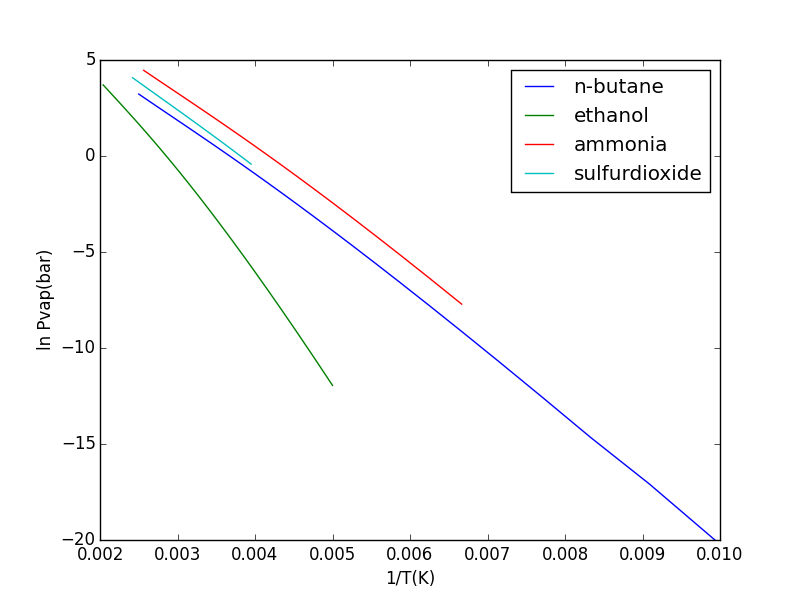
\includegraphics[width=0.75\textwidth]{my-plot.png}
\caption{\label{fig:fig2} Vapor pressure (bar) vs temperature (K) for four selected substances, computed using the PR equation of state.}
\end{figure}

\fi

\end{enumerate}

\end{document}
